\documentclass{article}
\usepackage[english]{babel}
\usepackage[utf8]{inputenc}
\usepackage{amsmath,amssymb}
\usepackage{parskip}
\usepackage{graphicx}
\graphicspath{ {./MA3210_images/} }

\newcommand\tab[1][1cm]{\hspace*{#1}}

% Margins
\usepackage[top=2.5cm, left=3cm, right=3cm, bottom=4.0cm]{geometry}


\title{MA3210 (Analysis II)}
\author{Jia Cheng}
\date{September 2021}

\begin{document}

\maketitle

\section{Definitions}
\paragraph{Sets}
\begin{align*}
	\mathbb{N}=\mathbb{Z}^+
\end{align*}

\section{Inequalities}
\begin{itemize}
	\item $|a + b| \leq |a| + |b|$
	\item $||a| - |b||\leq |a - b|$
	\item $||a| - |b|| = ||a| - |-b|| \leq |a + b|$
\end{itemize}

\section{Techniques}
\paragraph{Infimum and supremum}
Let $A, B$ be 2 sets of real numbers.\\
Given that $\forall a\in A, \exists b\in B, a\leq b$ we want to show $\sup A \leq \sup B$.\\
There are in general 2 ways to do this.

The direct way is to go from $B$ to $A$. Take arbitrary $a\in A$, then $\exists b\in B, a\leq b\leq \sup B$. Then $\sup B$ is an upper bound of $A$, hence $\sup A\leq \sup B$. We call this going from $B$ to $A$ in the sense that we produce $\sup B$ before producing $\sup A$ in our equations.

The other way goes in the reverse direction. Choose arbitrary $\epsilon>0$, and by definition of supremum, $\exists a\in A$, $\sup A - \epsilon<a\leq \sup A$. Again, there is a $b$ such that $\sup A-\epsilon < a\leq b\leq \sup B$. Hence $\sup A-\epsilon < \sup B$. Since $\epsilon$ is arbitrary, $\sup A\leq \sup B$.

Perhaps a better mnemonic for these 2 ways is that the first goes from the \textit{not pointy} bit of the inequality sign to the \textit{pointy} bit.

\section{Theorem Listing}
\subsection{Inf and sup}
\paragraph{Scalar properties}
Given a bounded set $S\subset \mathbb{R}$
\begin{align*}
\inf(cS)=
\begin{cases}
c\inf(S) \text{ if }c>0\\
c\sup(S) \text{ if }c<0
\end{cases}\\
\sup(cS)=
\begin{cases}
c\sup(S) \text{ if }c>0\\
c\inf(S) \text{ if }c<0
\end{cases}\\
\end{align*}

\paragraph{sup-inf condition}
Let $S$ be a nonempty bounded subset of $\mathbb{R}$ and $K>0$ such that $\forall s,t\in S,|s-t|\leq K$. Then $\sup(S)-\inf(S)\leq K$.

\subsection{Continuity}
\paragraph{Lipschitz property implies uniform continuity}
Lipschitz property: There is a constant $K$, such that for all $x,y$, $|f(x)-f(y)|\leq K|x-y|$.\\
It is then trivial to derive uniform continuity.

\subsection{Differential Calculus}
\paragraph{Caratheodory's Theorem}
Let $f: I\rightarrow \mathbb{R}$, $c\in I$. Then $f'(c)$ exists iff there is a function $\phi: I\rightarrow \mathbb{R}$ such that $\phi$ continuous at $c$ and
\begin{align*}
	\forall x\in I, f(x)-f(c) = \phi(x)(x-c)
\end{align*}
When this is the case, $\phi(c) = f'(c)$.

\paragraph{Inverse Function Lemma}
Let $f:I\rightarrow \mathbb{R}$ be strictly monotone and continuous on $I$. Let $J=f(I)$ such that $f^{-1}:J\rightarrow \mathbb{R}$ inverts $f$ (technically, we need to restrict the codomain of $f$ and $f^{-1}$ to just their range). Suppose $f$ differentiable at $c$ and $f'(c)\neq 0$. Then let $d=f(c)$ and
\begin{align*}
	(f^{-1})'(d) = \frac{1}{f'(f^{-1}(d)} = \frac{1}{f'(c)}
\end{align*}

\paragraph{Taylor's Theorem}
\begin{align*}
	f(x) = \sum_{k=0}^n\frac{f^{(k)}(a)}{k!}(x-a)^k + \frac{f^{(n+1)}(c)}{(n+1)!}(x-a)^{n+1}
\end{align*}

\subsection{Integral Calculus}
\paragraph{Properties of Riemann Integral}
\begin{itemize}
	\item Linearity
	\item Order-preserving $f\leq g\implies \int_a^b f\leq \int_a^b g$
	\item $f$ integrable implies $|f|$ integrable
	\item Triangle inequality
	\item Product of integrable functions is integrable
	\item Additive theorem: $\int_a^b f = \int_a^c f + \int_c^b f$
\end{itemize}

\paragraph{Fundamental Theorem of Calculus}
\subparagraph{FTC 2}
If $f: [a,b]\rightarrow \mathbb{R}$ is integrable and $f$ continuous at $c\in [a,b]$, then
\begin{align*}
	\frac{d}{dx}\int_a^xf |_{x=c} = f(c)
\end{align*}

\subparagraph{FTC 1}
If $g: [a,b]\rightarrow \mathbb{R}$ differentiable on $[a,b]$ and $g'$ integrable on $[a,b]$, then
\begin{align*}
	\int_a^bg' = g(b)-g(a)
\end{align*}

\paragraph{Integration by parts}
Suppose functions $f,g:[a,b]\rightarrow \mathbb{R}$ are differentiable on $[a,b]$, and $f',g'\in R([a,b])$. Then
\begin{align*}
	\int_a^b fg' = f(b)g(b)-f(a)g(a)-\int_a^b f'g
\end{align*}


\paragraph{Integration by substitution}
Suppose $\phi: [a,b]\rightarrow I$ is differentiable on $[a,b]$ and $\phi'\in R([a,b])$. Suppose $f: I\rightarrow \mathbb{R}$ continuous on $I$, then
\begin{align*}
	\int_a^b f(\phi(t))\phi'(t)\,dt = \int_{\phi(a)}^{\phi(b)}f(x)\,dx
\end{align*}
Note: To do "inverse substitution", we can start from the right side and find a suitable $\phi$ with the above mentioned characteristics. It doesn't need to be invertible, but we need to find $a,b$ such that $\phi(a), \phi(b)$ are the lower and upper limits on the RHS.

\paragraph{Taylor's Theorem Integral Form}
Let $f:[a,b]\rightarrow \mathbb{R}$. Suppose $\forall x\in (a,b)$, $f^(n+1)$ exists on $[a,x]$ and $f^{(n+1)}\in R([a,x])$. Then,
\begin{align*}
	f(x) = \sum_{k=0}^n\frac{f^{(k)}(a)}{k!}(x-a)^k + \frac{1}{n!}\int_a^xf^{(n+1)}(t)(x-t)^n\,dt
\end{align*}

\paragraph{Equivalence Theorem}
Let $f:[a,b]\rightarrow \mathbb{R}$ be bounded. $f$ is Darboux integrable iff $f$ is Riemann integrable.

\paragraph{Infinite Series}
Suppose $f$ is Riemann/Darboux integrable and we have a sequence of partitions $(P_n)$ of $[a,b]$ as well as accompanying choice functions $\gamma_n$ such that $\lim_{n\rightarrow \infty}||P_n||=0$.
Then
\begin{align*}
	\lim_{n\rightarrow \infty} S(f, P_n)(\gamma_n) = \lim_{||P||\rightarrow 0} S(f, P)(\gamma) = \int_a^bf
\end{align*}

Note that the $\gamma_n$ are truly arbitrary, the important thing is that $||P_n||\rightarrow 0$


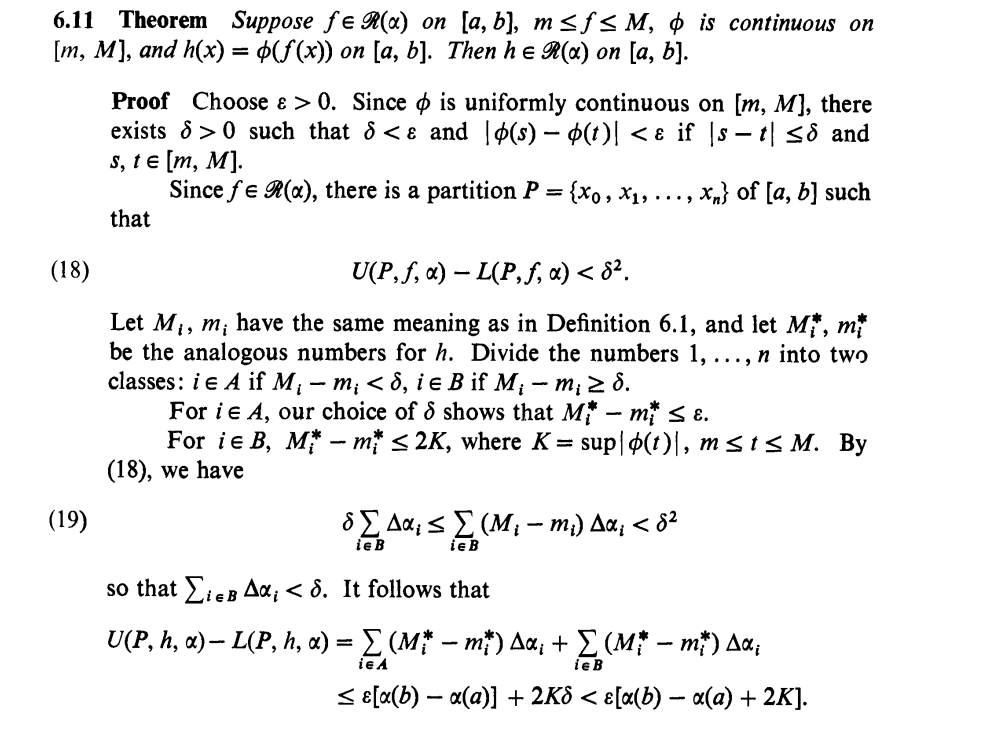
\includegraphics[scale=0.8]{theorem_6_11}

\end{document}


